By approximating \eqref{eq:LognormalBlueReal} and
\eqref{eq:LognormalBlueImag} one can gain some more insight about the
spectral density and the smallest/largest eigenvalues. First we note that the
denominator in \eqref{eq:LognormalBlueImag} behaves approximately like
a step function as shown in figure \ref{fig:BlueDenominator}. In
section \ref{sec:eigen_M}/\ref{sec:eig_m} we investigate the mean
of the largest/smallest eigenvalue, for which the case of $x>0$
respective $x<0$ is relevant.

\begin{figure}[htb!]
  \centering
  \subfigure[x = -0.3, y = -0.5, q = 0.7]{
    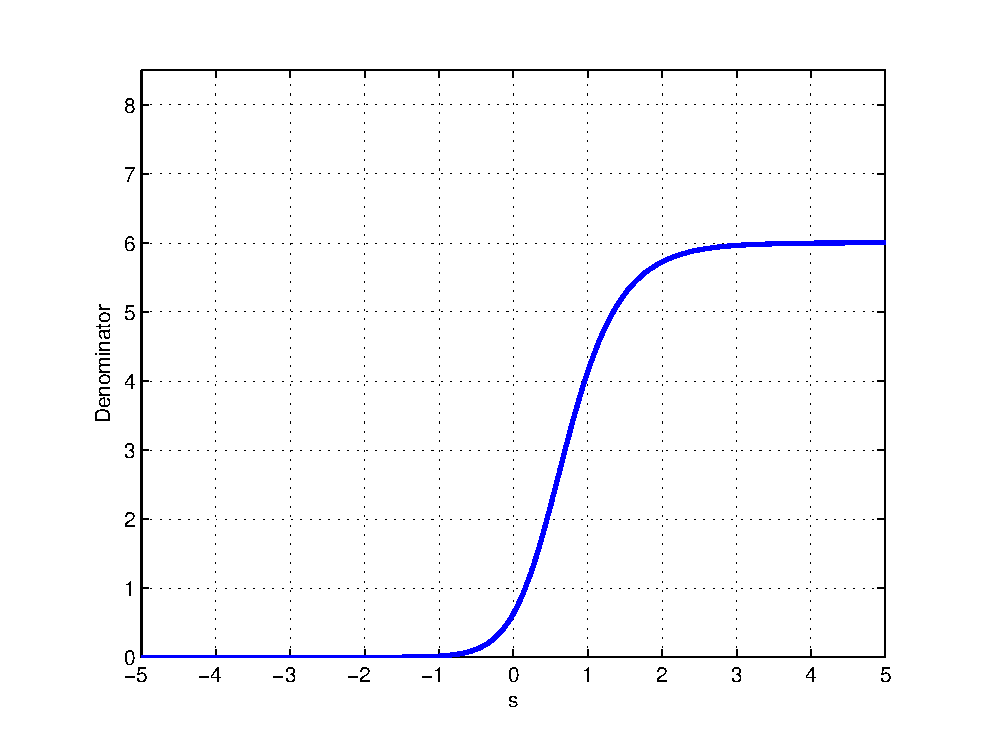
\includegraphics[scale=0.35]{../pics/LognormalBlueDe1.eps}
    \label{fig:LognormalBlueDe1}
  }
  \subfigure[x = 0.3, y = -0.5, q = 0.7]{
    \includegraphics[scale=0.35]{../pics/LognormalBlueDe2.eps}
    \label{fig:LognormalBlueDe2}
  }
  \caption{\small \it Plot of the function
    $\frac{
      1
    }{
      (e^{-2s} - qx)^2 + q^2 y^2  
    }$}
  \label{fig:BlueDenominator}
\end{figure}

\section{Large Eigenvalues}\label{sec:eigen_M}
From figure \ref{fig:LognormalBlue} one can see that, when $\re B$ has
large values, $\re G > 0$. In this case the reciprocal of the 
denominator in \eqref{eq:LognormalBlueImag}, i.e. $\frac{1}{(e^{-2s} -
  qx)^2 + q^2   y^2}$, is plotted in figure \ref{fig:LognormalBlueDe2}.
Clearly, this function attains its maximum at $s_1 = -{1 \over
  2}\log(qx)$. Depending in on the values of $qx$, we approximate
\eqref{eq:LognormalBlueReal} and \eqref{eq:LognormalBlueImag} in
different ways. These are detailed in the following sections.

\subsection{very small Re G}
When the real part of the Green's function (denoted $x$) is much smaller than $1/q$
such that $s_1$ is far to the right, we Taylor-expand $\frac{1}{(e^{-2s} -
  qx)^2 + q^2   y^2}$ in \eqref{eq:LognormalBlueImag} around
$e^{2s}=1$ to the first order, and then integrate it with $e^{-s^2/2v}
ds \over \sqrt{2\pi v}$ over $s \in [-2v,2v]$. This yields
\begin{equation}\label{eq:eigmax1}
\frac{q \text{erf}\left(\sqrt{2} \sqrt{v}\right)}{q^2 y^2+(1-q
  x)^2}+\frac{2 q \left(\frac{1}{2} e^{2 v} \text{erf}\left(2 \sqrt{2}
      \sqrt{v}\right)-1\right) (1-q x)}{\left(q^2 y^2+(1-q
    x)^2\right)^2} = {1 \over x^2 + y^2}
\end{equation}
Similarly, we Taylor-expand $e^{-2s}-qx \over (e^{-2s}-qx)^2 + q^2y^2$
in \eqref{eq:LognormalBlueReal}, which is plotted in figure
\ref{fig:BlueRealDenPos}, and integrate over the same interval 
to obtain
\begin{equation}\label{eq:eigmax2}
\lambda = \frac{\text{erf}\left(\sqrt{2} \sqrt{v}\right) (1-q x)}{q^2 y^2+(1-q
    x)^2}+\frac{\left(\frac{1}{2} e^{2 v} \text{erf}\left(2 \sqrt{2}
        \sqrt{v}\right)-1\right) \left((1-q x)^2-q^2
      y^2\right)}{\left(q^2 y^2+(1-q x)^2\right)^2} + {x \over x^2 + y^2}
\end{equation}
\begin{figure}[htb!]
  \centering
  \includegraphics[scale=0.6]{../pics/BlueRealDen.eps}
  \caption{\small \it Plot of the function
    $e^{-2s}-qx \over (e^{-2s}-qx)^2 + q^2y^2
    $. x = 0.5, y = -0.1, q = 0.5
  }
  \label{fig:BlueRealDenPos}
\end{figure}
For convenience, we employ the following symbols
\begin{eqnarray}
  \zeta &=& {1 - qx \over (1-qx)^2 + q^2y^2} \label{eq:eigmax6}\\
  \rho^2 &=& (1-qx)^2 + q^2y^2  \label{eq:eigmax7}\\
  a &=& \text{erf}(\sqrt{2v})  \label{eq:eigmax8} \\
  b &=& 1-{1 \over 2}e^{2v}\text{erf}(\sqrt{8v})  \label{eq:eigmax9}
\end{eqnarray}
This way $\rho$ can be eliminated using \eqref{eq:eigmax1}:
\begin{equation}\label{eq:eigmax3}
  {1 \over \rho^2} = {q \over a - 2b\zeta} +2\zeta -1
\end{equation}
Rewriting \eqref{eq:eigmax2} and inserting \eqref{eq:eigmax3} gives
\begin{equation}\label{eq:eigmax4}
  \lambda = -2b\zeta^2 + (a+2b)\zeta + {bq \over a-2b\zeta} - b
\end{equation}
Now we determine the range of $\zeta$. Since $x$ is assumed to be much
less than $1/q$ and hence $1 - qx > 0$, it is clear from
\eqref{eq:eigmax6} that $\zeta > 0$. In addition,
\begin{equation*}
  \zeta = \frac{1-q x}{q^2 y^2+(1-q x)^2} < \frac{1}{1-qx} < \frac{1}{1-qx_\M}
\end{equation*}
where by assumption $x_\M \ll 1/q$. Moreover, \eqref{eq:eigmax1} leads to
\begin{eqnarray*}
  2bq\zeta &=& aq - \frac{q^2 y^2+(1-q x)^2}{x^2+y^2} \\
  \zeta &=& {a \over 2b} - {1 \over 2bq}\frac{q^2 y^2+(1-q x)^2}{x^2+y^2}
\end{eqnarray*}
Since
\begin{equation*}
  \frac{q^2 y^2+(1-q x)^2}{x^2+y^2} >
  \frac{q^2 y^2+(1-q x_\M)^2}{x_\M^2+y^2} > 0
\end{equation*}
we have
\begin{itemize}
\item if $b > 0$, 
  \begin{equation*}
    0 < \zeta < \min\{{a \over 2b} - {1 \over 2bq}\frac{q^2 y^2+(1-q
      x_\M)^2}{x_\M^2+y^2}, \frac{1}{1-qx_\M}\}
  \end{equation*}
\item if $b < 0$,
  \begin{equation*}
    \max\{{1 \over 2|b|q}\frac{q^2 y^2+(1-q
      x_\M)^2}{x_\M^2+y^2}-\frac{a}{2|b|}, 0\} < \zeta < \frac{1}{1-qx_\M}
  \end{equation*}
\end{itemize}
We see that $\zeta$ is bounded to positive finite values and also
bounded away from $a/2b$ when $b > 0$. So \eqref{eq:eigmax4} suggests
$\lambda$ is finite. Solving \eqref{eq:eigmax4} for $\zeta$ gives
\begin{equation}
  \label{eq:eigmax12}
  \zeta = {1 \over 6b^2} \left\{
    2b(a+b) + \frac{b^2[a^2+2 a b-2 b (b+3
      \lambda)]}{[f(\lambda) + g(\lambda)]^{1/3}} + [f(\lambda) +
    g(\lambda)]^{1/3}\right\}
\end{equation}
where
\begin{eqnarray}
  f(\lambda) &=& -a^3 b^3-3 a^2 b^4+15 a b^5+9 a b^4 \lambda -10
  b^6-18 b^5 \lambda -27 b^5 q \label{eq:eigmax10} \\
  g(\lambda) &=& b^3 \left\{[a^3+3 a^2 b-3 a b (5 b+3
        \lambda )+b^2 (10 b+18 \lambda +27 q)]^2-\right. \nonumber \\
    && \left.[a^2+2 a b-2 b (b+3 \lambda )]^3\right\}^{1/2} \label{eq:eigmax11}
\end{eqnarray}
When $x \ll 1/q$, $1-qx \approx 1$. So we may write
\begin{eqnarray*}
  \zeta &\approx& {1 \over q^2 y^2 + 1} \\
  |y| &\approx& {1 \over q}\sqrt{{1 \over \zeta} - 1}
\end{eqnarray*}
Inserting \eqref{eq:eigmax9}, \eqref{eq:eigmax10} and
\eqref{eq:eigmax11} into the above equation gives an approximate
expression for $|y|$ and hence the spectral density $|y|/\pi$.

\subsection{Re G close to 1/q}
% So, as an approximation of the integral in
% \eqref{eq:LognormalBlueReal2}, one may neglect contributions from
% beyond $s_1$. Meanwhile, the contribution from the left of $s_1$ may
% be approximated by the integration of an exponential function:
% \begin{eqnarray*}
% \lambda &=& -{1 \over 2}\left({x \over y}-1\right)\int_{-\infty}^{s_1} e^{2s -
%   s^2/2v} {ds \over \sqrt{2\pi v}} + {x \over x^2 + y^2}
% \end{eqnarray*}
% where the factor $-{1 \over 2}\left({x \over y}-1\right)$ has been
% multiplied so that the approximating function $-{1 \over 2}\left({x
%     \over y}-1\right) e^{2s}$ and the original function
% $\frac{1}{\frac{q^2 y^2}{e^{-2 s}-q x}+\left(e^{-2 s}-q x\right)}$
% have the same value at $s_1$. Evaluating the above integral gives
% \begin{eqnarray}
% \lambda &\approx& -{1 \over 2}e^{2v}\left(
%   {x \over y} - 1 \right)+ \frac{x}{x^2 + y^2} \label{eq:LargestEig2}
% \end{eqnarray}
% In summary, the problem of the largest eigenvalue is the problem of
% maximizing \eqref{eq:LargestEig2} with the constraint
% \eqref{eq:LargestEig1}. Rewrite \eqref{eq:LargestEig1} as
% \begin{eqnarray*}
%   \left({-x^2 \over y}\right)^2 + x^2 &=& {e^{-8v} \over q}
% \end{eqnarray*}
% and introduce an angle $0<\theta \ll 1$ such that
% \begin{eqnarray*}
%   -\frac{x^2}{y} &=& {e^{-4s} \over \sqrt{q}} \cos\theta \\
%   x &=& {e^{-4s} \over \sqrt{q}} \sin\theta
% \end{eqnarray*}
% Then
% \begin{eqnarray}
%   \lambda &=& {1\over 2} e^{2v} (\cot\theta + 1) + {\cos^2\theta \over {e^{-4s}
%       \sin\theta / \sqrt{q}}} \label{eq:LargestEig3}
% \end{eqnarray}
% Clearly $\lambda$ diverges as $\theta \to 0$. To see how fast it
% diverges in relation to how fast $y \to 0$, we express $\theta$ as
% \begin{eqnarray*}
%   \theta &=& \cos ^{-1}\left(\sqrt{\frac{1}{4} q e^{8 v}
%       y^2+1}+\frac{1}{2} \sqrt{q} e^{4 v} y\right)
% \end{eqnarray*}
% Then \eqref{eq:LargestEig3} becomes
% \begin{equation}\label{eq:LargestEig4}
% \lambda = \frac{\xi ^2 \sqrt{q} e^{4 v}}{\sqrt{1-\xi ^2}}+\frac{1}{2}
% \left(\frac{\xi }{\sqrt{1-\xi ^2}}+1\right) e^{2 v}
% \end{equation}
% where
% \begin{equation*}
%   \xi = \sqrt{\frac{1}{4} q e^{8 v} y^2+1}+\frac{1}{2} \sqrt{q} e^{4
%     v} y
% \end{equation*}
% Neglecting terms of higher orders than $y$, $\xi$ is simply
% \begin{equation}\label{eq:LargestEig5}
%   \xi = \frac{1}{2} \sqrt{q} e^{4 v} y+1
% \end{equation}
% Similarly $\sqrt{1-\xi ^2}$ can be expanded as
% \begin{equation}\label{eq:LargestEig6}
%   \sqrt{1-\xi ^2} \approx e^{2v} q^{1/4} (-y)^{1/2}
% \end{equation}
% Inserting \eqref{eq:LargestEig5}, \eqref{eq:LargestEig6} into
% \eqref{eq:LargestEig4} and omitting positive powers of $-y$ gives
% \begin{equation*}
%   -\lambda +\frac{1}{2} \frac{1}{\sqrt[4]{q}} u^2+\sqrt[4]{q} u e^{2
%     v}+\frac{e^{2 v}}{2} = 0
% \end{equation*}
% where $u = (-y)^{-1/4}$. The positive root of this equation is
% \begin{equation*}
%   -y = \left(
% \sqrt{2 \sqrt[4]{q} \lambda - \sqrt[4]{q} e^{2 v}+q e^{4
%     v}}-\sqrt{q} e^{2 v}\right)^{-4} 
% \end{equation*}

\section{Small Eigenvalues}\label{sec:eig_m}
% \section{L\'evy innovations \& lognormal volatilities with AR(1)
%   autocorrelation}
% We shall find the S-transform of $\bm{\bar{\sigma}^2}$ using
% \eqref{eq:greens} and insert it into \eqref{eq:S_E} to find the
% S-transform of $\bm E$, which then leads to the Green's function as
% well as the spectral density of $\bm E$. When $\log\sigma \sim
% N\left(0, 1/(1 - \phi^2)\right)$
% \begin{eqnarray*}
%   G_{\bar{\sigma}^2}(z) &=& \mean{\frac{1}{z - \sigma^2}}\\
%    &=& \int_{-\infty }^{\infty } \frac{\exp \left(-\frac{s^2}{2
%       v}\right)}{\sqrt{2 \pi  v} \left(z-e^{2 s}\right)} \, ds
% \end{eqnarray*}
% where $v = 1/(1 - \phi^2)$. Evaluating this
% integral analytically is difficult, so we make an approximation and
% neglect contributions from large $|s|$, i.e. restrict the integration
% to a small interval $[-a, a]$ with $0 < a < 1$. Under this
% approximation, we Taylor-expand $e^{-s^2/2v}$ and $e^{2s}$ around 0
% and obtain
% \begin{eqnarray*}
%   G_{\bar{\sigma}^2}(z) &\approx& \int_{-a}^a \frac{1-s^2/2v}{\sqrt{2
%       \pi  v} (z-1-2 s)} \, ds \\
%   &=&\frac{8 v \log \left(\frac{-2 a-z+1}{2 a-z+1}\right)+(z-1)
%     \left(4 a+(z-1) \left(2 \coth ^{-1}\left(\frac{2 a}{1-z}\right)+i
%         \pi \right)\right)}{16 \sqrt{2 \pi }
%     v^{3/2}} \label{eq:G_sigma}
% \end{eqnarray*}
% The moment generating function $M_{\bar{\sigma}^2}(z)$ follows as
% $zG_{\bar{\sigma}^2}(z) - 1$. Inverting $M_{\bar{\sigma}^2}(z)$ gives
% the S-transform
% \begin{eqnarray*}
%   S_{\bar{\sigma}^2}(z) &=& {1 - z \over z M^{-1}_{\bar{\sigma}^2}(z)}
% \end{eqnarray*}
% \eqref{eq:G_sigma} is a transcendental equation and can be solved only
% numerically.
\section{temp}
\begin{table}[htb!]
  \centering
  \begin{tabular}{c|c|c|c|c}
    & Tail func. & $\lambda_c$ & Extrapolated fraction ($\lambda >
    \lambda_c$) & counted fraction ($\lambda > \lambda_c$) \\
    \hline
    v = 0.25 & ${100 / \lambda^{6.3}}$ & 15.8 & $2.59\times 10^{-6} $ &
    $3.86 \times 10^{-6}$ \\
    \hline
    v = 0.5 & ${20 / \lambda^{3.14}}$ & 100 & $1.0471\times 10^{-5}$ &
    $7.57\times 10^{-6}$ \\
    \hline
    v = 0.75 & $38.46/\lambda^{2.5}$ & 398 & $1.24 \times 10^{-5}$ &
    $1.19 \times 10^{-5}$ \\
    \hline
    v = 0.9973 & $29.52/\lambda^{1.98}$ & 1000 & $3.42 \times
    10^{-5}$ & $2.55 \times 10^{-5}$ \\
    \hline
    v = 1.0 & $24.26/\lambda^{1.94}$ & 1000 & $3.69 \times 10^{-5}$ &
    $2.50 \times 10^{-5}$ \\
    \hline
    v = 1.99 & $21.38/\lambda^{1.19}$ & 39811 & $7.31 \times 10^{-5}$ &
    $1.80 \times 10^{-5}$ \\
  \end{tabular}
  \caption{Num. large eigenvalues. T/K=10}
  \label{tab:tab1}
\end{table}
